\chapter{An M.Sc.\ Student Remembers GR}\label{chap18}

\Authorline{G Umesh\footnote[*]{Email: \url{umesh52@gmail.com}}}
\addtocontents{toc}{\protect\contentsline{section}{{\sl G Umesh}\smallskip}{}}

\authinfo{Retired Professor of Physics, NITK Surathkal}


After completing B.Sc.(Hons) in 1973, with just an average First Class from Bangalore University, I was keenly looking for an opportunity to join the University of Mysore for M.Sc.\ In those days there was only one seat available for graduates of Universities other than Mysore. I had obtained admission for M.Sc.\ at Central College, Bangalore, and had paid up the Fee to join there. In the meantime, I was offered admission to the Physics Department at Manasagangothri ! My joy knew no bounds and I immediately joined University of Mysore. The Physics Department at Manasagangothri had a formidable reputation, specially the four Professors who led the group of faculty members in teaching the four major domains in which any student could specialize for the M.Sc.\  degree, viz. Nuclear Physics, Solid State Physics, Spectroscopy and Theoretical Physics. I entered the Classroom meant for the first-year students with a great sense of awe and expectations. Unlike the UG Colleges, we now had an entire building housing the Physics Department with sufficient rooms for teaching and Laboratories. The space surrounding the Department building was also equally salubrious with so many large Banyan trees! The Department was well served by about 20 faculty members. Right from day one, I felt a great difference in the atmosphere between an undergraduate College and a post graduate Department! This feeling was further strengthened when Prof.\ K. N. Srinivasa Rao held the first class. He taught us Classical Mechanics in the first year. He began by saying  ``All that you have learnt about Classical Mechanics so far in your earlier classes has many errors. You have to learn it afresh right from the fundamentals”!! And so, he began describing the philosophical questions which the ancient Greeks, such as Zeno, had posed! I was mesmerized by the amount of knowledge revealed by KNS in each class that he took for us. For the first time we were being exposed to the ideas that formed the foundations of Physics. Other subjects were taught very well by Prof.\ P. Venkataramaiah, Prof.\ J. Shashidhara Prasad, Dr.\ H. S. Subramaniam (HSS), Dr.\ K. S. Puttaswamy and Dr.\ S. Gopal. I used to marvel at the amount of information HSS would give us in each class on atomic spectroscopy without using any Notes! The first year was a great learning experience for me. I recall the great friendliness shown towards us students by not only the faculty members but also the senior students in the Department. The welcome party given to us by our seniors set the tone for a relationship that has lasted till today! There was no sign of ``Ragging" when we entered the Department! In turn we too hosted a grand Farewell Party for our seniors at the end of our first year! The first year was also the time when we all classmates, including the girls, became very good friends and that has continued to this day! We make it a point to get together without fail on occasions like wedding celebrations of our children and greatly enjoy exchanging anecdotes of our M.Sc.\ days, talking about events of our past life and each other's welfare!
\vskip 2pt

Somewhere in the middle of 1973, a new faculty member joined the Department as Reader. He was Dr.\ G. Ramachandran who was quite young then. He started teaching the 7 or 8 senior students who had opted to specialize in Theoretical Physics! Within a short time, we came to know that here was another Star Teacher! I had made up my mind in the beginning of the first year to opt to specialize in Theoretical Physics. Having been placed 7th in the order of merit in the first-year examination, I was a bit jittery that I may not be offered Theoretical Physics. However, some of my fellow classmates changed their minds and I got into the Theoretical Physics Group without any problems. Then started a year of exhilarating education for me in Physics!! The four stalwarts who taught us theory courses were Prof.\ K. N. Srinivasa Rao, Prof.\ G. Ramachandran, Dr.\ A. V. Gopala Rao and Dr.\ C. K. Venkatanarasimhaiah; we students lovingly called them KNS, GR, AVG and CKV. Others who taught us were Prof.\ B. Sanjeevaiah (then HOD), Dr.\ K. Gopala, Prof.\ D. Krishnamurthy and Dr.\ H. Sanjeevaiah. The courses taught to us Theoretical Physics students were so intense that we had to be on our toes always. A close friend of mine Dr.\ S. A. Prasad, who was also two years senior to me, told me at that time that by the end of the second year, we would have a fairly good idea of the state of art in each subject taught to us!! He had said that we would be well equipped to take up research immediately after M.Sc.! Many a time I have wished that we should have had one more year of M.Sc.\ to completely absorb the amount of knowledge to which we were exposed. I must add that the learning experience was more enjoyable due to the excellent camaraderie among us classmates! We greatly enjoyed each other's company and shared our experiences and troubles. Several of us were inmates of the PG Hostel with all its kinks! Many classmates were staying in the Village Hostel and other private hostels. Our camaraderie continues to this day and we have a WhatsApp Group too. Recollecting the days spent at Manasagangothri during 1973--75 gives us immense happiness and contentment!
\vskip 2pt

Now a little more about our Theoretical Physics batch of 1974--75. Prof.\ KNS was a formidable teacher. He taught us Group Theory and its applications in Physics. He started from the basics of Set Theory, which I must reveal, we were learning for the first time! He had an excellent handwriting on the Blackboard, and he would write practically every important statement and mathematical steps on the Board. I still remember the beautiful way he would use the Blackboard space while lecturing. In each class, from start to finish, I would be furiously noting down as much of what he spoke as possible for me; my handicap was that I was not fast in writing. The challenge in his class was to absorb what he spoke in addition to noting down at the same time at a fast pace! Looking back, I must say that it was sheer poetry at its best delivered non-stop in each class! I really wish we had a third year of M.Sc.\ In contrast AVG's classes were not so fast paced and he would also speak, in measured tone, more slowly than KNS. He taught us Tensor Analysis and then General Theory of Relativity. His style of writing on the black board was remarkably similar to that of KNS. I learnt many things about the beauty of Mathematics from KNS and AVG. I could take down the lectures more comfortably in AVG's class. I must also mention that on a couple of occasions, AVG would write down more on the Black Board, speak less and look at us expectantly to see if we have grasped the points written on the Board! He was extraordinarily meticulous in his teaching and would repeat certain intricate aspects in the next class. From him I learnt the importance of doing Maths properly! Dr.\ CKV taught us Plasma Physics and Fluid Mechanics. He had a style of his own and would relate many anecdotes and make the subjects attractive. I remember he was very fond of bringing in Bogadi Village into his stories. I remember him as a very friendly teacher with whom we were very comfortable!
\vskip 2pt

Dr.\ GR was an entirely different personality!! Our comfort level was maximum in his classes. He taught us Quantum Mechanics and High Energy Physics. We always found him smiling and would often laugh aloud heartily after telling us anecdotes or stories. We would have most of his classes in the afternoon and they would stretch to 2--3 hours and more! I must say we had no complaints against the extended classes since it was so enthralling. GR would also derive all the equations and solutions on the spot without using any written Notes! I remember very well, that after deriving many a result or clarifying a concept, GR would say ``There is nothing very profound about it ...." and then go on to explain a deeper concept, thereby drawing our attention to the ``wheat" as against the  ``chaff”! Although the text book used for the course on Advanced Quantum Mechanics was the book authored by Paul Roman, GR would often refer us to many other books such as the ones written by L. I. Schiff, M. E. Rose, Bjorken and Drell, Dirac, etc. Besides, he would often give us Technical Reports published by Laboratories like CERN, SLAC and BNL, to read and enjoy! However, I recall that the University Library was rather poorly equipped, and we had quite some problems in getting access to textbooks on the topics being taught. There was a small Library in the Department which was of some help. I clearly recall that we depended mainly on whatever we wrote down in our copies during the lectures. This was particularly true of the Mathematics topics taught by KNS and AVG! I also remember very clearly that one of my seniors told me to go and purchase a copy of the book on Mathematical Physics by G. Arfken from Geetha Book House in the city before the copies get sold out! To my good luck I was able to buy it but learning from this book was quite a task. Later in my career, I came across the book by E. Kreyszig on Engineering Mathematics and found it to be a delightful book for self-study. I must also admit that I was very carefree during those days of my life and, therefore, did not absorb as much of Physics as I could have from such wonderful teachers as GR, KNS and AVG. Lack of sufficient good books was a major impediment for self-learning during the 1970s. Compared to those days, the present times are vastly different with the availability of a large number of excellent books, Video lectures on YouTube by stalwarts, Tutorials, E-Books and above all internet access to a variety of reading/learning materials. The scope for self-learning any topic through internet has revolutionized education these days. One may even say that this is an age of  ``information overload" with the associated consequences!     

An important event in the 2$^{\rm nd}$ year of M.Sc.\ for the students of Theoretical Physics Group was the Seminar that each one of us had to give. All our four Professors and our classmates would be the audience. This event was more like an open examination and, hence, we would be very nervous on the D-Day. GR had asked me to speak on Einstein's Coefficients of emission and absorption of light. I remember he had suggested that I look up books on Lasers! I did not have the faintest idea about Lasers and could not get any book on Lasers; perhaps I did not search for a book hard enough. I was the first student to give the seminar and due to the poor preparation, I did not do a satisfactory job. So, I had to repeat the seminar on another day! I also remember that our classmate Nagesh Rao had to talk about Superfluidity and he did an excellent job! His seminar was greatly appreciated.

The employment scenario in the country in early 1970s was rather bleak. Among my classmates (about 45 students) only about 6 or 7 joined for Ph.D. in different institutions. Many of my classmates joined Banks and P\&T Department of the Government. My thinking was to join for Ph.D. in experimental Physics. However, I did not have any definite idea about the research area or the institution to join. There was very little time to consult someone or explore the existing possibilities. I joined IIT, Delhi, for Ph.D. simply because I could stay with my parents in New Delhi. Very interestingly, I ended up doing research on theoretical aspects of Laser-Plasma Interactions! In fact, I had no intentions of working in the field of Plasma Physics and, as chance would have it, I had to study the basics of Lasers as well as the physics of Plasmas. It took more than a year for me to get on track. What excited me about this research area was that it was directly related to controlled Nuclear Fusion for energy generation! I have often kicked myself for not taking the M.Sc.\ seminar topic on Lasers seriously. I should say that the well equipped Library at IIT Delhi made a big difference to me in my education. I must also add that the opportunity to attend lectures by eminent Physicists who visited IIT Delhi and the seminars/lectures delivered by the Professors and Research Students in the Department was a great source of inspiration. When I joined for Ph.D. in June 1975, there were more than 90 Research Scholars in the Physics Department working on a wide variety of topics. We could attend the Ph.D. defence seminar of any student in the Department. This open atmosphere of interaction across the research Groups in various Departments made research activity very enjoyable. Added to this was the Computer Centre where we could carry out large computations related to our work. Looking back, I am of the opinion that creating an environment similar to that in the 5 older IITs would go a long way in promoting research activities in Indian Universities. I now realize that GR set up exactly such an environment in his research Group at Manasagangothri!

After completing my Ph.D. in 1979, I continued to serve in IIT Delhi till December 1991. Then I shifted to Karnataka Regional Engineering College (KREC), Surathkal, in January 1992. I served this Institute, now known as National Institute of Technology Karnataka (NITK) till January 2017, when I finally got retired. At NITK the emphasis was on teaching Under-graduate Engineering students. So much of my time was taken up teaching two courses in each semester. I also initiated research on Fiber Optic devices in a limited way. Many B.Tech.\ and M.Tech.\ students worked on final year Projects under my supervision right from the start in 1992. These activities became fruitful mainly due to my education at the University of Mysore for M.Sc.\ and the exposure to research at IIT Delhi. The teaching methods of Prof.\ KNS, Prof.\ GR and Prof.\ AVG have always guided me in my teaching. Further, I have been greatly influenced by the approach to research in applied physics that I witnessed at IIT Delhi. From my thesis advisor Prof.\ M. S. Sodha, I imbibed the spirit of indulging in research in inter-disciplinary areas. I have greatly enjoyed doing this at NITK. From Prof.\ A. K. Ghatak and Prof.\ K. Thyagarajan I learnt the art of teaching Physics to students in a class and of mentoring Research Scholars in their work.  

I had the unique opportunity to supervise the Ph.D. research of Mr.Vikas Shelar along with Prof.\ GR as the Co-Guide!! In fact this student had already worked with GR's younger brother Mr.G.Visvanathan, who was a scientist at ISRO, for about a year or so. This student worked on Flow Visualization in high speed gas dynamics by applying spectroscopic techniques; Vikas had a good background in spectroscopy. We were lucky to get the opportunity to carry out most of the experiments at the Aerospace Engineering Department, Indian Institute of Science, Bengaluru, using the Shock Tube facility. They were interested in developing the spectroscopic techniques for their own experiments. This work required a proper understanding of the physics of fluorescence and it was GR who taught us how to compute the cross-sections for such phenomena in molecular gases. This collaboration resulted in a couple of good papers in Journals on spectroscopy and Vikas earned his Ph.D. in the year 2014. Currently, Dr.\ Vikas Shelar is an Assistant Professor in the Physics Department at Ramaiah University of Applied Sciences, Bengaluru.

From October 2013 till December 2014, I served the Central University of Karnataka at Kalaburgi (then called Gulbarga) on deputation from NITK, Surathkal. The then Vice Chancellor of CUK, Prof.\ S. S. Murthy, requested Director of NITK to send me on deputation to CUK for 1 or 2 years. CUK, which had started functioning from the Campus of Gulbarga University from 2009, had started M.Sc.\ Degree programs in Physics, Chemistry and Mathematics in 2012 and there was acute shortage of qualified faculty in the fledgling University. When I joined the Physics Department at CUK, there were only two part-time faculty members in the Department, and I was the third! We had students in both 1$^{\rm st}$ year and 2$^{\rm nd}$ year M.Sc., and it was a huge challenge to carry on with the teaching commitments. The senior students were in great stress since the teaching in the 1$^{\rm st}$ year was rather poor. We had to request many Professors from other Institutions to come and teach as Guest Faculty. To our good fortune many renowned Professors agreed to help us out and teach different segments of the syllabus! Prof.\ GR also agreed to teach Quantum Mechanics through Online Video Lectures. He was not in a position to travel to Gulbarga due to poor health. He delivered about 10 lectures in the available time. However, due to logistics issues we could not continue his Lectures in the subsequent semesters. We managed to complete the 1$^{\rm st}$ semester of the academic session July – December, 2013. In the meantime, interviews were held in November 2012, to recruit new faculty members in all the Departments in the University. To our good fortune we were able to select three excellent candidates for the Physics Department, namely, Dr.\ Rajeev Joshi, Dr.\ Bharat Kumar and Dr.\ Deepak Samuel. In January 2013, CUK shifted to its own Campus, located 30km outside Kalaburgi, on the highway to Aland. Since then there has been a steady growth in the academic activities in the University. The three faculty members have built up the Physics Department admirably well through sheer hard work. Several graduates of the Physics Department have joined Ph.D. programs in reputed Universities in India and abroad. I am happy to say that the contribution of GR to this success story was invaluable!

I met GR several times at his home in Bengaluru. He always received me warmly and with a broad smile. We would mostly discuss some aspects of Physics and ways to teach the topics better. He would also tell me about several events that happened in his illustrious career at I.M.Sc.\ Chennai and Mysore University and, after retirement, at I.I.A. Bengaluru. Sometime in 2007, his younger brother Sri G.Visvanathan, who was working at ISTRAC (ISRO), suggested that we should submit a Research Project to DST to establish a Polarimetric Microwave Radar Facility on the Campus of NITK to monitor the South-West Monsoon on the western coast. The Project was planned as collaboration between NITK and ISTRAC with Prof.\ G. Ramachandran as a Co-investigator. With GR's guidance we were to develop the theoretical model for scattering of polarized microwave radiation from clouds with the aim of understanding the Monsoon phenomena better. The budget for the Project was close to Rs.4.00 crores and, perhaps for this reason, it was not granted. Had it been granted, we would have built a unique experimental facility for cloud monitoring on the western coast of India.

Starting from my days as a student of M.Sc., I have learnt much from my interactions with GR. This was possible due, mainly, to his friendliness towards all his students and his simplicity. I have not seen him get angry at anyone. I have never felt any hesitation in going to his home to meet him and such visits would usually last a few hours. After my retirement in January 2017, I had plans to meet him more often and work on electromagnetic wave scattering using the formalism of density matrix. GR had advised me to study his famous Report on Angular Momentum published by I.M.Sc.\ and I obtained a copy of it from the Library of I.M.Sc.\ Due to domestic issues I could not invest sufficient time for this study. I still plan to study the Report with the help of friends who have been students of GR!

It is very difficult to absorb the permanent absence of GR from our midst. I was aware of the gradual deterioration in his health over the last couple of years, but I was hoping that he would be around for several more years. I met him last in the middle of December 2019 when I went to invite him to my son's wedding and sought his blessings. Soon after the wedding ceremony COVID-19 caught up with all of us. It has inflicted tragedy on so many of us and continues to affect our lives. My last meeting with GR is still fresh in my mind. I will cherish his blessings for the rest of my life!
\vskip 1cm

\centerline{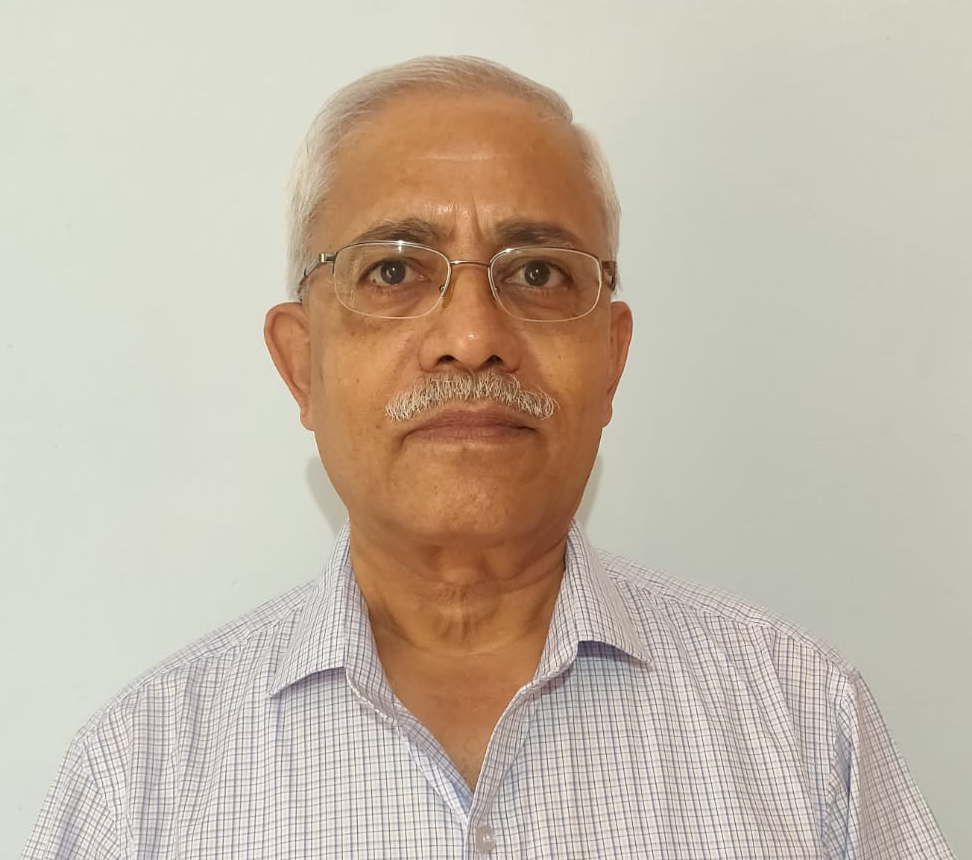
\includegraphics[scale=0.15]{authorsphotos/G_Umesh.jpg}}
\bigskip

\noindent
\textbf{Dr.\ G. Umesh} obtained the M.Sc.\ degree from Physics Department, Mysore University, in 1975, and  Ph.D. from IIT Delhi, in 1979. He joined Physics Department, IIT Delhi, in 1981 and worked there till 1991. He then joined Physics Department, NITK, Surathkal, in 1992 and retired from there in January, 2017. Currently he leads an active retired life at Mysuru.

\begin{center}
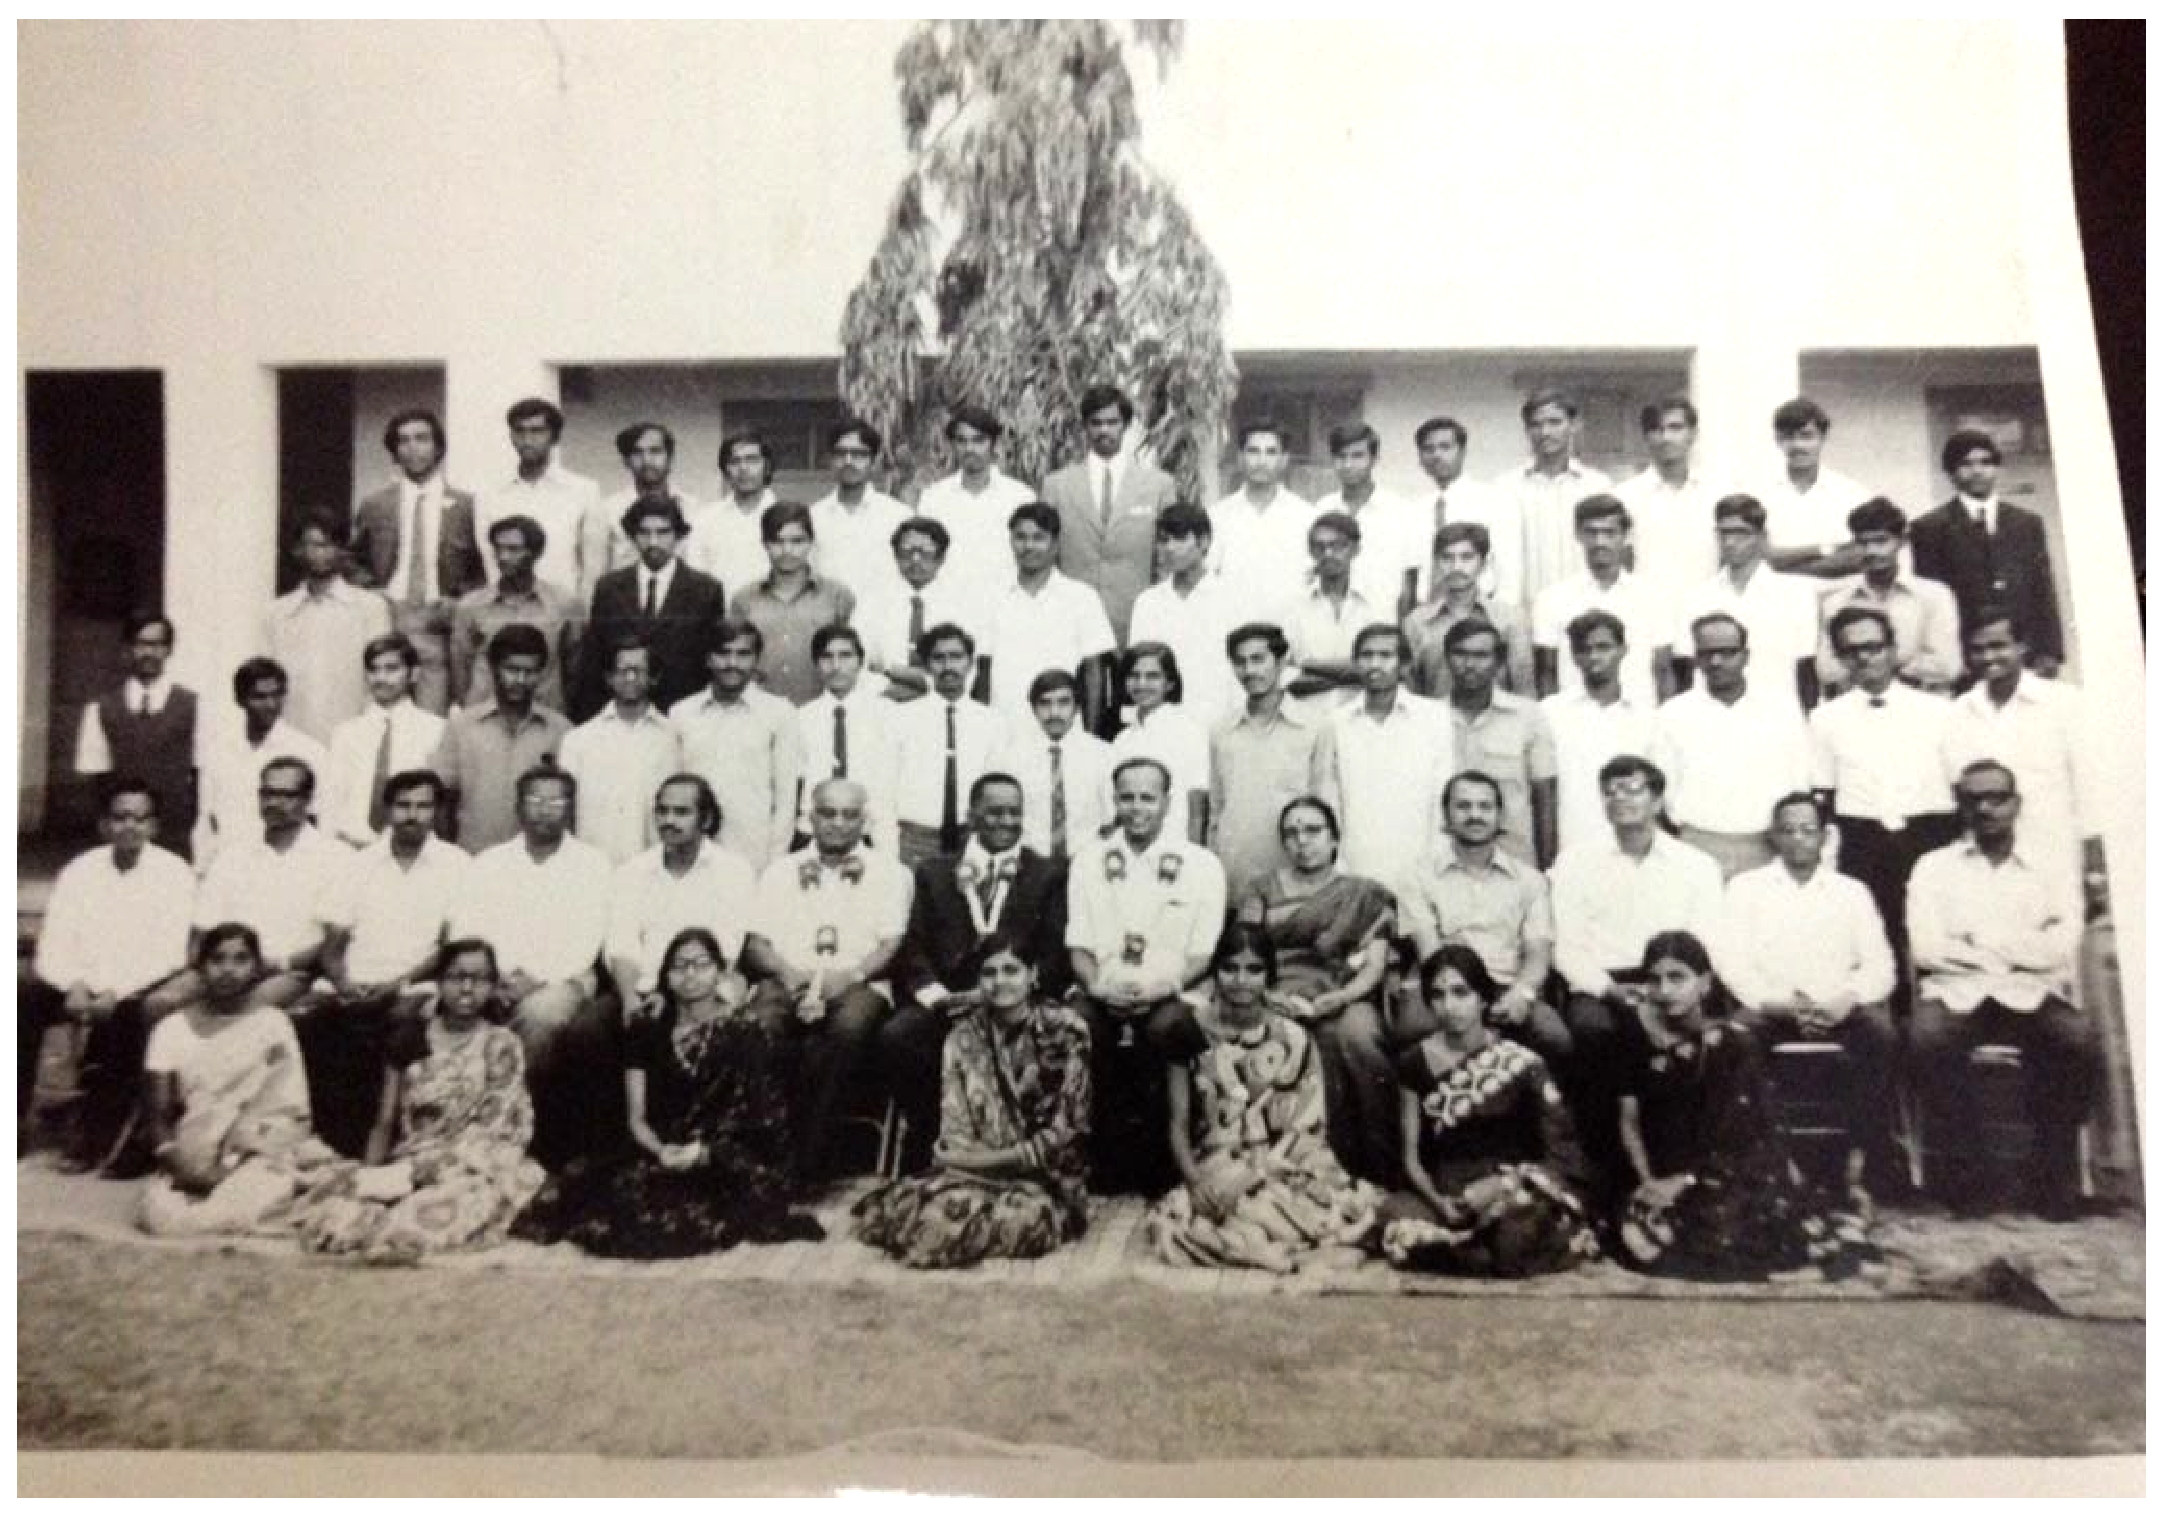
\includegraphics[scale=0.278]{src/images/chap8/8.eps}\\[3pt]
M.Sc.\ Final year students (batch of 1975, DOS in Physics, University of Mysore) 
with their Professors. Prof.\ G R is seated on the chair first from the left.
\end{center}
